% ============================================================
%  sec-3-ascend-ecosystem.tex  —  2.3 Huawei Ascend Ecosystem
% ============================================================

\section{Huawei Ascend Ecosystem}
\label{sec:ascend-ecosystem}

The Huawei Ascend ecosystem implements a full-stack AI computing
infrastructure based on DaVinci architecture \acrshort{npu}s, the CANN
runtime and compiler layer, the MindSpore framework, and the ModelArts
cloud platform. This vertically integrated stack enables hardware-software
co-design for optimal AI workload execution across device, edge, and cloud
deployment scenarios — and constitutes the primary hardware target of
this project.

\begin{figure}[H]
    \centering
    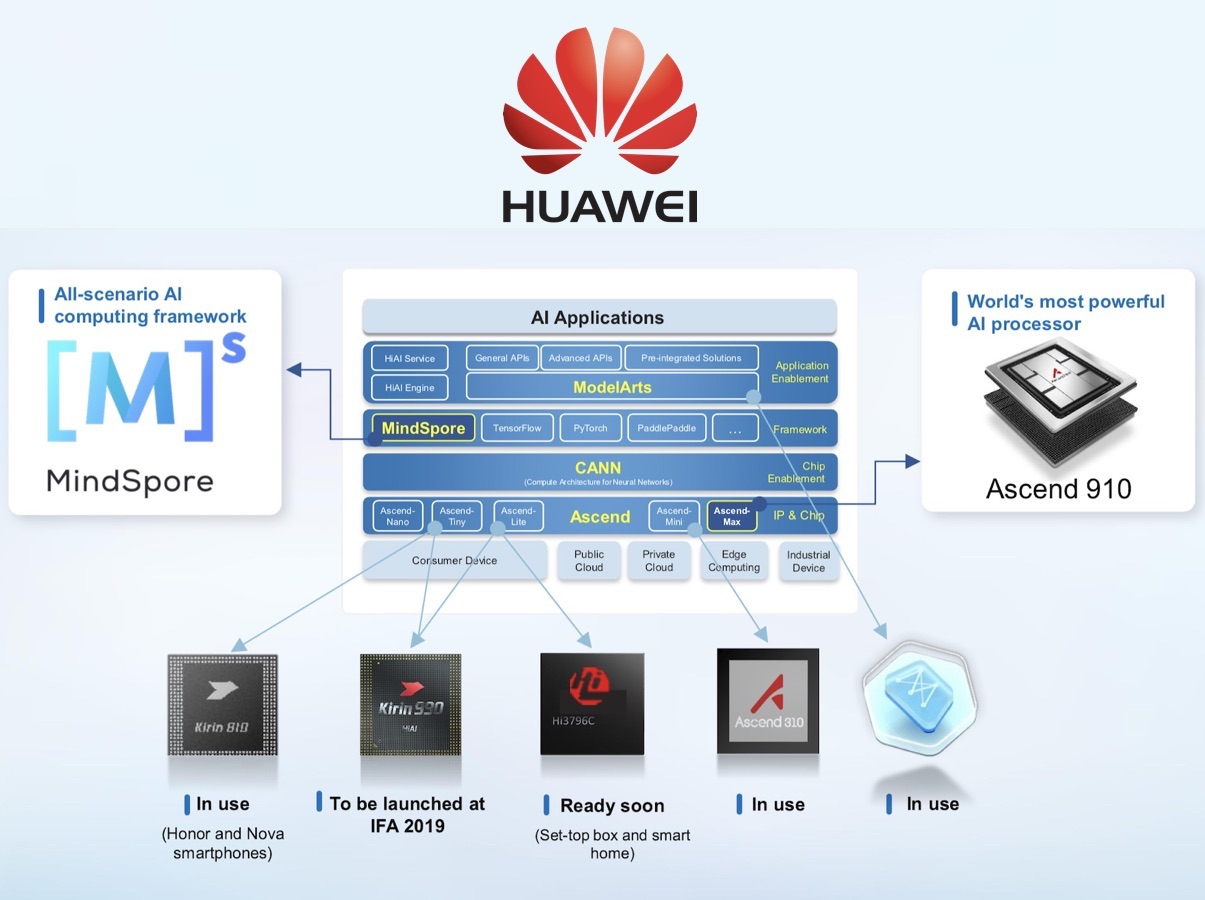
\includegraphics[width=0.7\textwidth]{images/figures/huaweiAIecosystem.jpg}
    \caption{Huawei AI Ecosystem}
    \label{fig: Huawei AI Ecosystem}
\end{figure}

% ── 2.3.1 ────────────────────────────────────────────────────
\subsection{Ascend Hardware Architecture}
\label{subsec:ascend-hw}

\subsubsection{DaVinci Core Architecture}

Huawei Ascend \acrshort{npu}s implement the DaVinci architecture, a
3D computational design consisting of three specialised processing units
per core:

\begin{table}[htbp]
  \centering
  \caption{DaVinci core computational units}
  \label{tab:davinci-units}
  \begin{tabularx}{\textwidth}{llXX}
    \toprule
    \tableheader{Unit & Dimensionality & Function & Operations/Cycle} \\
    \midrule
    Cube Unit   & 3D ($16\times16\times16$) & Matrix multiply-accumulate & 4,096 FP16 MACs + 8,192 INT8 MACs \\
    \rowcolor{TableRowOdd}
    Vector Unit & 2D (2,048-bit)            & Activation functions, element-wise & 2,048-bit INT8/FP16/FP32 \\
    Scalar Unit & 1D                        & Control flow, address generation   & Full flexibility, branch logic \\
    \bottomrule
  \end{tabularx}
\end{table}

The Cube Unit performs the fundamental 3D matrix operation
$D = A \times B + C$ where $A$, $B$, $C$, $D$ are all $16 \times 16$
matrices, yielding 4,096 parallel FP16 MAC operations in a single cycle.
The Vector Unit handles 2,048-bit wide activation and normalisation operations.
The Scalar Unit manages control flow and address generation, enabling the
Cube and Vector units to operate in pure dataflow mode.

\subsubsection{Ascend 910 Chip Specifications}

\begin{table}[htbp]
  \centering
  \caption{Huawei Ascend 910 key specifications}
  \label{tab:ascend-910-specs}
  \begin{tabularx}{0.9\textwidth}{lX}
    \toprule
    \tableheader{Parameter & Specification} \\
    \midrule
    AI Cores           & 32 DaVinci cores \\
    \rowcolor{TableRowOdd}
    FP16 Performance   & 256 TFLOPS/s @ 1.0 GHz \\
    INT8 Performance   & 512 TOPS \\
    \rowcolor{TableRowOdd}
    On-Chip SRAM       & 84 MB total (32 MB shared buffer) \\
    Memory             & 32 GB HBM2 via 4 channels \\
    \rowcolor{TableRowOdd}
    Memory Bandwidth   & 1,228 GB/s off-die \\
    Process Node       & 7nm+ EUV \\
    \rowcolor{TableRowOdd}
    TDP                & 300–350 W \\
    Interconnects      & PCIe 3.0 $\times$16, HCCS, 100G RoCE \\
    \bottomrule
  \end{tabularx}
\end{table}

The 32 DaVinci cores are organised in a mesh topology connected by the
CHIE Network-on-Chip (NOC). Each core has independent L0 buffers
(64 KB A + 64 KB B + 256 KB Unified), a 1 MB L1 buffer, and shares a
32 MB global buffer across all cores. Memory transfers between levels
are managed by the dedicated Memory Transfer Engine (\acrshort{mte}).


% ── 2.3.2 ────────────────────────────────────────────────────
\subsection{CANN Runtime Architecture}
\label{subsec:cann}

\acrfull{cann} is Huawei's heterogeneous computing architecture providing
the runtime, compiler, and operator library layer between AI frameworks
and Ascend hardware — the direct analogue of NVIDIA's \acrshort{cuda}
stack.

\begin{figure}[H]
    \centering
    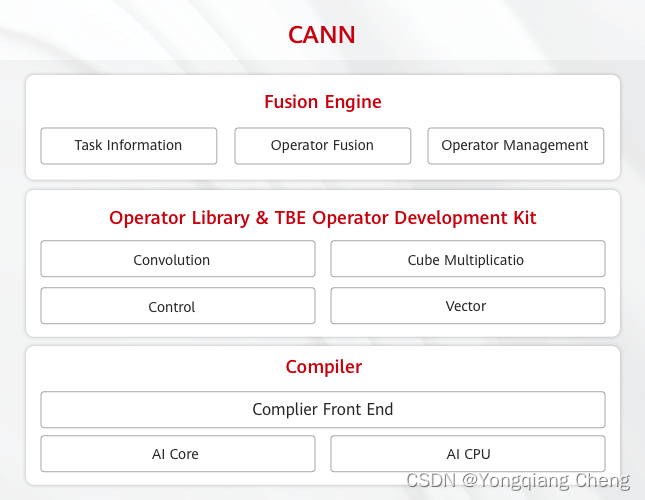
\includegraphics[width=0.7\textwidth]{images/figures/CANN-architecture.png}
    \caption{CANN Architecture Overview}
    \label{fig: CANN Architecture Overview}
\end{figure}

\subsubsection{Layered Architecture}

CANN is organised into two abstraction layers. \textbf{L1 (CANN)} is
the architecture-dependent layer providing hardware abstraction, task
scheduling, and the AscendCL API. \textbf{L2 (Graph Engine)} is
the architecture-independent optimisation layer performing operator
fusion, cross-layer memory optimisation, and compute-communication
parallelism.

AscendCL (Ascend Computing Language) is the unified programming interface
analogous to CUDA's runtime API, covering device and context management,
host-device memory transfers, model loading (from compiled \texttt{.om}
files), and stream-based asynchronous execution.

\subsubsection{Compiler Stack}

\begin{table}[htbp]
  \centering
  \caption{CANN compiler stack components}
  \label{tab:cann-compiler}
  \begin{tabularx}{\textwidth}{llX}
    \toprule
    \tableheader{Component & Input → Output & Function} \\
    \midrule
    Graph Compiler & IR → Hardware executable & Converts framework IR to Ascend executable \\
    \rowcolor{TableRowOdd}
    TBE (Tensor Boost Engine) & Operator → kernel & Auto-schedules efficient operator compilation \\
    OMG (Offline Model Generator) & Framework model → \texttt{.om} & Converts Caffe/TF/MindSpore to DaVinci offline model \\
    \bottomrule
  \end{tabularx}
\end{table}



% ── 2.3.3 ────────────────────────────────────────────────────
\subsection{MindSpore Execution Framework}
\label{subsec:mindspore}

MindSpore is Huawei's all-scenario AI framework supporting device-edge-cloud
deployment. It employs Source Code Transformation (\acrshort{sct}) for
automatic differentiation:
\begin{equation}
  \text{Function} \xrightarrow{\text{SCT}} \text{IR}
  \xrightarrow{\text{Parse}} \text{Computational Graph}
  \label{eq:sct}
\end{equation}

MindSpore offers a unified graph mode that switches seamlessly between
static execution (pre-compiled, production-optimised) and dynamic execution
(immediate, research-friendly) — a design advantage over PyTorch's separation
between eager and TorchScript modes.

In distributed training, MindSpore supports three parallel strategies
(data, model, hybrid) with an automatic parallelism search that explores
a large strategy space — contrasting with PyTorch's manual
\texttt{DistributedDataParallel} configuration.

\subsubsection{Performance}

The MindSpore + Ascend 910 combination achieves 1,802 images/second on
ResNet-50 V1.5 (ImageNet 2012) — approximately $2\times$ the throughput
of the mainstream TensorFlow + GPU baseline (965 img/s). This performance
advantage stems from MindSpore's native CANN integration eliminating the
translation overhead that external frameworks incur.


% ── 2.3.5 ────────────────────────────────────────────────────
\subsection{Ascend AI System Stack: End-to-End Integration}
\label{subsec:ascend-stack}

The four layers of the Ascend stack form a cohesive execution path from
user-facing AI code to hardware compute:

\begin{table}[htbp]
  \centering
  \caption{Full Ascend AI system stack}
  \label{tab:ascend-stack}
  \begin{tabularx}{\textwidth}{llX}
    \toprule
    \tableheader{Layer & Component & Primary Function} \\
    \midrule
    L4 & ModelArts      & AI lifecycle management, distributed training orchestration, MLOps \\
    \rowcolor{TableRowOdd}
    L3 & MindSpore      & Computational graph execution, automatic differentiation, parallelism \\
    L2 & CANN           & Graph optimisation, operator fusion, hardware abstraction, AscendCL API \\
    \rowcolor{TableRowOdd}
    L1 & Ascend (DaVinci) & Tensor computation via Cube/Vector/Scalar units \\
    \bottomrule
  \end{tabularx}
\end{table}

An important engineering caveat: MindSpore-native models achieve
$\approx 2\times$ the throughput of PyTorch/TensorFlow running on Ascend
via CANN, which incurs 10–20\% translation overhead. For production
systems targeting Ascend hardware, the native MindSpore path is strongly
preferred; frameworks migrated from the CUDA ecosystem must weigh this
performance cost against the effort of framework-level code changes.
